\chapter{The Container Loading Problem}
\section{Formal Problem Definition}
\section{Computational Complexity and NP-hardness}
\section{Constraints in the CLP}
\section{Related Problems: Bin Packing, Knapsack, Cutting Stock}

The placement and assignment of three-dimensional items to larger, mostly rectangular
containers, is a well known problem in logistics and operations research, as the
potential of cost savings and efficiency gains is substantial by reducing the number
of needed containers or by fulfilling customer needs. These problems are differentiated
by \cite{bortfeldt_constraints_2013} in \textit{input minimization}, where the number
of needed containers is minimized, and \textit{output maximization} problems, where the
value of the associated items is maximized.

Differentiate the Multiple Container Loading Problem, from Knapsack problem,
and cutting stock problem \parencite{bortfeldt_constraints_2013}

Use systemization of \parencite{bortfeldt_constraints_2013} to group problems in
groups

Define Items, and how they are meant here. Differnetiate between heterogenous
and homogenous items.

Define the container.

\begin{figure}[H]
    \centering
    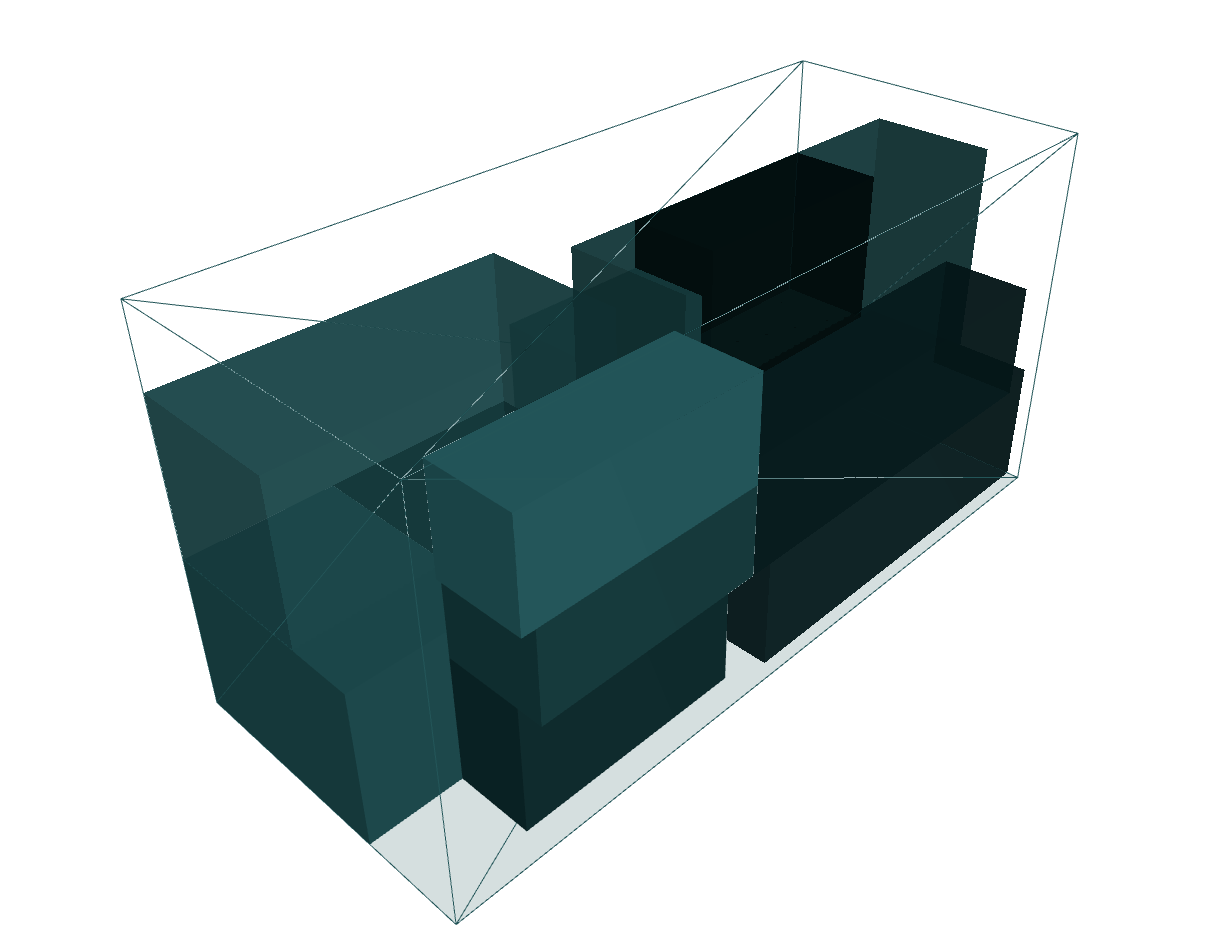
\includegraphics[width=7cm]{pictures/3l_cvrp_example.png}
    \caption{Visualization from \cite{tamke_branch-and-cut_2024}.}
    \label{fig:solution-visualization}
\end{figure}